\section{1. BH定理}

\begin{frame}[allowframebreaks=] 
 \frametitle{}
 定理一: 如果两算符满足
 \[[A,[A,B]] = [B, [A,B]]=0\]
 则有 
 \[e^{A+B}= e^A e^B e^{-\frac{1}{2}[A,B]} =  e^B e^A e^{\frac{1}{2}[A,B]}\]  
 \证~令 $ f(\xi) = e^{\xi A} e^{\xi B}$ 
\[ \begin{aligned}
    \frac{\mathrm{d}f}{\mathrm{d}\xi} &=Ae^{\xi A} e^{\xi B} + e^{\xi A} Be^{\xi B} \\
    &= Ae^{\xi A} e^{\xi B} + e^{\xi A} Be^{\xi B} e^{-\xi A} e^{-\xi B} e^{\xi A} e^{\xi B} \\
    &= (A+e^{\xi A} Be^{-\xi A})e^{\xi A} e^{\xi B} \\ 
    &= (A+e^{\xi A} Be^{-\xi A}) f(\xi)
\end{aligned}\] 
      
令 $g(\xi)= e^{\xi A} Be^{-\xi A}$, 并做泰勒展开
\[\begin{aligned}
        g(\xi) &= g(0)+ \xi \frac{\mathrm{d}g}{\mathrm{d}\xi}|_{\xi=0}+ \frac{1}{2!}\xi^2 \frac{\mathrm{d}^2g}{\mathrm{d}\xi^2}|_{\xi=0}+ \cdots \\ 
        &= B + e^{\xi A}[A,B]e^{-\xi A}|_{\xi=0} + e^{\xi A}[A,[A,B]]e^{-\xi A}|_{\xi=0} + \cdots \\ 
        &= B + \xi[A,B] \\ 
    \frac{\mathrm{d}f}{\mathrm{d}\xi} &= ((A+ B) + \xi[A,B] )f(\xi) \\ 
    \frac{\mathrm{d}f}{f(\xi)} &= ((A+ B) + \xi[A,B] ) \mathrm{d}\xi\\ 
    f(\xi) &=  e^{((A+ B)\xi + \frac{\xi^2}{2} [A,B] )}\\ 
    e^{\xi A} e^{\xi B} &= e^{(A+ B)\xi} e^{\frac{\xi^2}{2} [A,B]}
    \end{aligned} \]
    取 $\xi=1$, 得:
    \[e^{A+B}= e^A e^B e^{\frac{1}{2}[A,B]}\] 
    同理, 有 
    \[e^{A+B} = e^{B+A} = e^B e^A e^{\frac{1}{2}[B,A]} =e^B e^A e^{-\frac{1}{2}[A,B]} \] 
    证毕!
\end{frame}

\section{2. 相位算符}

\begin{frame} [allowframebreaks=] 
 \frametitle{}
      经典光场的复振幅 
      \[ a= \left|a\right| e^{i\varphi}\]
      经典光场的正则分量
      \[ q(t) = a e^{-\omega t} + a e^{\omega t} = 2\left|a \right|\cos(\omega t + \varphi)\]
      (1) 那是否可写出一个相位算符呢?, 比如把湮灭算符写成
      \[ \hat{a} = \hat{g} e ^ i \hat{\varphi} \]
      这种写法是不行的, 因为
      $e ^ i \hat{\varphi}$与$e ^ {-i \hat{\varphi}}$ 并不是幺正的, 会导致 $\hat{\varphi}$不是厄密的,因而没有可测量意义. \\ {\vspace*{0.3em}}
      (2) 为保证厄密, 有人定义了新的相位算符
      \[ \sin \hat{\varphi}, \cos \hat{\varphi}\]
      指数形式为
      \[\hat{C}= \frac{1}{2} [e^{i \hat{\varphi}} + e^{- i \hat{\varphi}}]\]
      \[\hat{S}= \frac{1}{2i} [e^{i \hat{\varphi}} - e^{- i \hat{\varphi}}]\]
      与产生湮灭算符有如下关系
      \[\hat{a}= \sqrt{\hat{N}+1}(\hat{C}+i\hat{S})\]
      \[\hat{a}^{\dagger}= (\hat{C}-i\hat{S})\sqrt{\hat{N}+1}\]
      但是, $\hat{C}, \hat{S}$不对易, 说明如果能描述相位,它们两也对应两个不同的相位.\\ 
      反向求得:
      \[ C= \]
      \[ Q= \]
\end{frame}

\section{3. 多模光场}

\begin{frame}[allowframebreaks=]  
 \frametitle{}
 多($l$)模光场的张量积(直积)描述\\ 
 真空态
 \[ \rs{0 }= \rs{00\cdots 0 } \] 
零点能
\[ E_0 = \sum_l \frac{1}{2} \hbar \omega_l\]
本征能
\[ E_n = \sum_l  \hbar \omega_l[\frac{1}{2}+ n_l]\]
本征态
\[\rs{n } =\rs{n_1 }\rs{n_2 }\cdots \rs{n_l }= \rs{n_1n_2  \cdots n_l } \]
哈密顿
\[ H = \sum_l \frac{1}{2} \hbar \omega_l(a^{\dagger}_l a_l + a_la^{\dagger}_l )\]
\[ a_l \rs{n } = \sqrt{n_l}\rs{n_1 }\rs{n_2 }\cdots \rs{n_{l}-1 } \]
态的展开式
\[ \rs{\psi} = \sum_{n_1, n_2, \cdots n_l} a_n \rs{n_1 }\rs{n_2 }\cdots \rs{n_{l}}\]
密度算符
\[ \rho = \prod_l \rho_l = \prod_l \sum_{n_l} P_{n_l}\rl{n_l}{n_l}
\]
\end{frame}

\begin{frame} 
 \frametitle{}
   例: 计算双模场算符Q的均值
   \[  Q= \Omega \sum_{i,j,k,l} a^{\dagger} _i a^{\dagger} _j a_k a_l, \qquad i,j,k,l =1,2 \]
   \[ \begin{aligned}
       \overline{Q}&= \left\langle n_1 n_2|Q|n_2n_1  \right\rangle \\
       &= \Omega[\left\langle n_1 n_2|a^{\dagger} _1 a^{\dagger} _1 a_1 a_1|n_2n_1  \right\rangle + \left\langle n_1 n_2|a^{\dagger} _1 a^{\dagger} _2 a_1 a_2|n_2n_1  \right\rangle \\ 
       & + \left\langle n_1 n_2|a^{\dagger} _1 a^{\dagger} _2 a_1 a_2|n_2n_1  \right\rangle  
       + \left\langle n_1 n_2|a^{\dagger} _2 a^{\dagger} _2 a_2 a_2|n_2n_1  \right\rangle]  \\
       &= \Omega [(n_1 ^2 -n_1) + (n_2 ^2 -n_2) +4n_1 n_2 ]
   \end{aligned}\]    
\end{frame}

\section{4. 相干函数}

\begin{frame} 
\frametitle{~4.1 经典相干函数}
     \begin{columns}
         \begin{column}[t]{0.69\linewidth}
      
         \end{column}
         \begin{column}[t]{0.3\linewidth} 
               \begin{center}
                    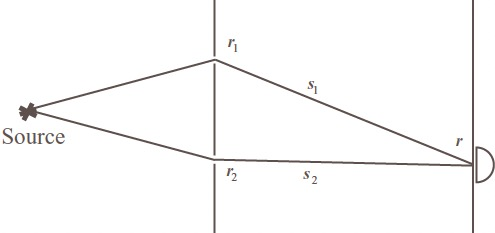
\includegraphics[width=1.0\textwidth]{figs/2022-06-02-14-02-17.png} 
               \end{center} 
         \end{column} 
     \end{columns} 
\end{frame}

